\documentclass[twoside]{book}

% Packages required by doxygen
\usepackage{fixltx2e}
\usepackage{calc}
\usepackage{doxygen}
\usepackage[export]{adjustbox} % also loads graphicx
\usepackage{graphicx}
\usepackage[utf8]{inputenc}
\usepackage{makeidx}
\usepackage{multicol}
\usepackage{multirow}
\PassOptionsToPackage{warn}{textcomp}
\usepackage{textcomp}
\usepackage[nointegrals]{wasysym}
\usepackage[table]{xcolor}

% Font selection
\usepackage[T1]{fontenc}
\usepackage[scaled=.90]{helvet}
\usepackage{courier}
\usepackage{amssymb}
\usepackage{sectsty}
\renewcommand{\familydefault}{\sfdefault}
\allsectionsfont{%
  \fontseries{bc}\selectfont%
  \color{darkgray}%
}
\renewcommand{\DoxyLabelFont}{%
  \fontseries{bc}\selectfont%
  \color{darkgray}%
}
\newcommand{\+}{\discretionary{\mbox{\scriptsize$\hookleftarrow$}}{}{}}

% Page & text layout
\usepackage{geometry}
\geometry{%
  a4paper,%
  top=2.5cm,%
  bottom=2.5cm,%
  left=2.5cm,%
  right=2.5cm%
}
\tolerance=750
\hfuzz=15pt
\hbadness=750
\setlength{\emergencystretch}{15pt}
\setlength{\parindent}{0cm}
\setlength{\parskip}{3ex plus 2ex minus 2ex}
\makeatletter
\renewcommand{\paragraph}{%
  \@startsection{paragraph}{4}{0ex}{-1.0ex}{1.0ex}{%
    \normalfont\normalsize\bfseries\SS@parafont%
  }%
}
\renewcommand{\subparagraph}{%
  \@startsection{subparagraph}{5}{0ex}{-1.0ex}{1.0ex}{%
    \normalfont\normalsize\bfseries\SS@subparafont%
  }%
}
\makeatother

% Headers & footers
\usepackage{fancyhdr}
\pagestyle{fancyplain}
\fancyhead[LE]{\fancyplain{}{\bfseries\thepage}}
\fancyhead[CE]{\fancyplain{}{}}
\fancyhead[RE]{\fancyplain{}{\bfseries\leftmark}}
\fancyhead[LO]{\fancyplain{}{\bfseries\rightmark}}
\fancyhead[CO]{\fancyplain{}{}}
\fancyhead[RO]{\fancyplain{}{\bfseries\thepage}}
\fancyfoot[LE]{\fancyplain{}{}}
\fancyfoot[CE]{\fancyplain{}{}}
\fancyfoot[RE]{\fancyplain{}{\bfseries\scriptsize Generated by Doxygen }}
\fancyfoot[LO]{\fancyplain{}{\bfseries\scriptsize Generated by Doxygen }}
\fancyfoot[CO]{\fancyplain{}{}}
\fancyfoot[RO]{\fancyplain{}{}}
\renewcommand{\footrulewidth}{0.4pt}
\renewcommand{\chaptermark}[1]{%
  \markboth{#1}{}%
}
\renewcommand{\sectionmark}[1]{%
  \markright{\thesection\ #1}%
}

% Indices & bibliography
\usepackage{natbib}
\usepackage[titles]{tocloft}
\setcounter{tocdepth}{3}
\setcounter{secnumdepth}{5}
\makeindex

% Hyperlinks (required, but should be loaded last)
\usepackage{ifpdf}
\ifpdf
  \usepackage[pdftex,pagebackref=true]{hyperref}
\else
  \usepackage[ps2pdf,pagebackref=true]{hyperref}
\fi
\hypersetup{%
  colorlinks=true,%
  linkcolor=blue,%
  citecolor=blue,%
  unicode%
}

% Custom commands
\newcommand{\clearemptydoublepage}{%
  \newpage{\pagestyle{empty}\cleardoublepage}%
}

\usepackage{caption}
\captionsetup{labelsep=space,justification=centering,font={bf},singlelinecheck=off,skip=4pt,position=top}

%===== C O N T E N T S =====

\begin{document}

% Titlepage & ToC
\hypersetup{pageanchor=false,
             bookmarksnumbered=true,
             pdfencoding=unicode
            }
\pagenumbering{alph}
\begin{titlepage}
\vspace*{7cm}
\begin{center}%
{\Large My\+Sh }\\
\vspace*{1cm}
{\large Generated by Doxygen 1.8.13}\\
\end{center}
\end{titlepage}
\clearemptydoublepage
\pagenumbering{roman}
\tableofcontents
\clearemptydoublepage
\pagenumbering{arabic}
\hypersetup{pageanchor=true}

%--- Begin generated contents ---
\chapter{M\+Y\+SH}
\label{index}\hypertarget{index}{}\hypertarget{index_intro}{}\section{Introduction}\label{index_intro}
An implementation example for reader-\/writers protocol, giving priority to readers.

The goal of this example is to
\begin{DoxyItemize}
\item create two or more readers,
\item create a writer
\item simlutate some reads and some writes on shared data following the reader-\/writers protol.
\end{DoxyItemize}

See \hyperlink{rws_8c_abf9e6b7e6f15df4b525a2e7705ba3089}{main } function to run the code.

\begin{DoxyDate}{Date}
06/05/2018 
\end{DoxyDate}
\begin{DoxyVersion}{Version}
0.\+1.\+0 
\end{DoxyVersion}
\begin{DoxyAuthor}{Author}
Luca Parolari 
\end{DoxyAuthor}

\chapter{File Index}
\section{File List}
Here is a list of all documented files with brief descriptions\+:\begin{DoxyCompactList}
\item\contentsline{section}{\hyperlink{read__and__skip_8c}{read\+\_\+and\+\_\+skip.\+c} \\*Main file }{\pageref{read__and__skip_8c}}{}
\end{DoxyCompactList}

\chapter{File Documentation}
\hypertarget{mysh_8cpp}{}\section{mysh.\+cpp File Reference}
\label{mysh_8cpp}\index{mysh.\+cpp@{mysh.\+cpp}}


file principale  


{\ttfamily \#include $<$stdio.\+h$>$}\newline
{\ttfamily \#include $<$string.\+h$>$}\newline
{\ttfamily \#include $<$stdlib.\+h$>$}\newline
{\ttfamily \#include $<$unistd.\+h$>$}\newline
{\ttfamily \#include $<$string$>$}\newline
{\ttfamily \#include $<$sys/wait.\+h$>$}\newline
Include dependency graph for mysh.\+cpp\+:
\nopagebreak
\begin{figure}[H]
\begin{center}
\leavevmode
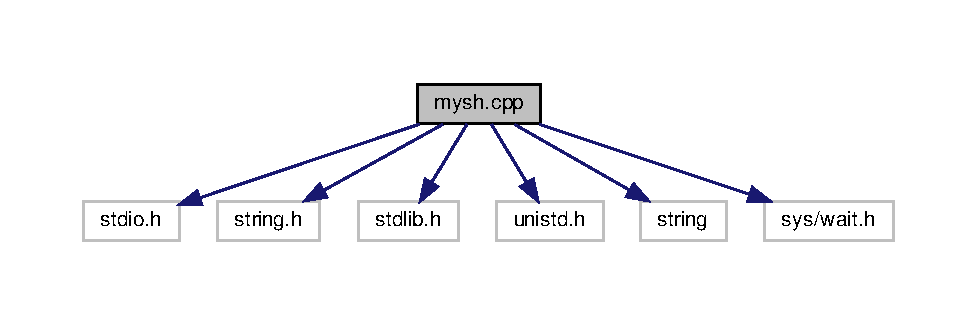
\includegraphics[width=350pt]{mysh_8cpp__incl}
\end{center}
\end{figure}
\subsection*{Macros}
\begin{DoxyCompactItemize}
\item 
\mbox{\Hypertarget{mysh_8cpp_a5fdce82727e278d6647e0addafcd6db6}\label{mysh_8cpp_a5fdce82727e278d6647e0addafcd6db6}} 
\#define \hyperlink{mysh_8cpp_a5fdce82727e278d6647e0addafcd6db6}{M\+A\+X\+P\+A\+R\+A\+MS}~6
\begin{DoxyCompactList}\small\item\em Numero elementi del vettore comando. \end{DoxyCompactList}\item 
\mbox{\Hypertarget{mysh_8cpp_a2d1edde91ea515b363277f4bbdc3244d}\label{mysh_8cpp_a2d1edde91ea515b363277f4bbdc3244d}} 
\#define \hyperlink{mysh_8cpp_a2d1edde91ea515b363277f4bbdc3244d}{M\+A\+X\+P\+A\+TH}~60
\begin{DoxyCompactList}\small\item\em Numero elementi del vettore P\+A\+TH. \end{DoxyCompactList}\end{DoxyCompactItemize}
\subsection*{Functions}
\begin{DoxyCompactItemize}
\item 
int \hyperlink{mysh_8cpp_aed1a95f1caee8dde3ade742565c4f0ec}{string2vpunt} (char $\ast$stringa, int maxchar, char $\ast$vpunt\mbox{[}$\,$\mbox{]}, int maxpunt, char $\ast$sep)
\begin{DoxyCompactList}\small\item\em Separa i tokens di una stringa in un vettore di puntatori. \end{DoxyCompactList}\item 
int \hyperlink{mysh_8cpp_a0db858019c02b516bf0266b3e945a88e}{vpunt\+\_\+print} (char $\ast$vpunt\mbox{[}$\,$\mbox{]})
\begin{DoxyCompactList}\small\item\em Stampa le stringhe da un vettore di puntatori. \end{DoxyCompactList}\item 
int \hyperlink{mysh_8cpp_a972c788e7fc092f962c7521e3012d198}{get\+\_\+command} (char $\ast$cmd\mbox{[}$\,$\mbox{]})
\begin{DoxyCompactList}\small\item\em Funzione per l\textquotesingle{}input e la gestione del comando. \end{DoxyCompactList}\item 
int \hyperlink{mysh_8cpp_a93f01522af4cf1259e6d3090b5c7aa7b}{esegui} (char $\ast$cmd\mbox{[}$\,$\mbox{]}, char $\ast$argv\mbox{[}$\,$\mbox{]}, char $\ast$envp\mbox{[}$\,$\mbox{]})
\begin{DoxyCompactList}\small\item\em Esegue il comando. \end{DoxyCompactList}\item 
int \hyperlink{mysh_8cpp_a93b17c8d56ff41f9fc389d7108e90d5e}{exec\+\_\+down} (char $\ast$vpunt\mbox{[}$\,$\mbox{]})
\begin{DoxyCompactList}\small\item\em Execute a command making a call to the down machine. \end{DoxyCompactList}\item 
int \hyperlink{mysh_8cpp_a61b9ac82f46fa513268fdf75eb298552}{command} (char $\ast$cmd, char $\ast$argv\mbox{[}$\,$\mbox{]})
\begin{DoxyCompactList}\small\item\em Execute a command using down machine. \end{DoxyCompactList}\item 
int \hyperlink{mysh_8cpp_aaf0b88b6765299395849c95fff004186}{which} (char $\ast$cmd, char $\ast$cmdfq)
\begin{DoxyCompactList}\small\item\em Search in paths the first occurence of target command, and returns the fully qualified name in cmdfq. \end{DoxyCompactList}\item 
int \hyperlink{mysh_8cpp_adedb285b02c41bde2158ded9cc9fd7ac}{main} (int argc, char $\ast$argv\mbox{[}$\,$\mbox{]}, char $\ast$envp\mbox{[}$\,$\mbox{]})
\begin{DoxyCompactList}\small\item\em Funzione principale. \end{DoxyCompactList}\end{DoxyCompactItemize}
\subsection*{Variables}
\begin{DoxyCompactItemize}
\item 
\mbox{\Hypertarget{mysh_8cpp_ab93cef35fe712f550f47256583a74376}\label{mysh_8cpp_ab93cef35fe712f550f47256583a74376}} 
char $\ast$ \hyperlink{mysh_8cpp_ab93cef35fe712f550f47256583a74376}{path} \mbox{[}\hyperlink{mysh_8cpp_a2d1edde91ea515b363277f4bbdc3244d}{M\+A\+X\+P\+A\+TH}\mbox{]}
\begin{DoxyCompactList}\small\item\em path Vettore di puntatori che verra\textquotesingle{} riempito con i P\+A\+TH \end{DoxyCompactList}\item 
\mbox{\Hypertarget{mysh_8cpp_a0bfc8700e33b89f73487f8b2b5528576}\label{mysh_8cpp_a0bfc8700e33b89f73487f8b2b5528576}} 
char $\ast$ \hyperlink{mysh_8cpp_a0bfc8700e33b89f73487f8b2b5528576}{comando} \mbox{[}\hyperlink{mysh_8cpp_a5fdce82727e278d6647e0addafcd6db6}{M\+A\+X\+P\+A\+R\+A\+MS}\mbox{]}
\begin{DoxyCompactList}\small\item\em comando Vettore comando\+: comando e opzioni \end{DoxyCompactList}\end{DoxyCompactItemize}


\subsection{Detailed Description}
file principale 

\begin{DoxyAuthor}{Author}
L. Parolari 
\end{DoxyAuthor}
\begin{DoxyDate}{Date}
31.\+05.\+18 
\end{DoxyDate}


\subsection{Function Documentation}
\mbox{\Hypertarget{mysh_8cpp_a61b9ac82f46fa513268fdf75eb298552}\label{mysh_8cpp_a61b9ac82f46fa513268fdf75eb298552}} 
\index{mysh.\+cpp@{mysh.\+cpp}!command@{command}}
\index{command@{command}!mysh.\+cpp@{mysh.\+cpp}}
\subsubsection{\texorpdfstring{command()}{command()}}
{\footnotesize\ttfamily int command (\begin{DoxyParamCaption}\item[{char $\ast$}]{cmd,  }\item[{char $\ast$}]{argv\mbox{[}$\,$\mbox{]} }\end{DoxyParamCaption})}



Execute a command using down machine. 


\begin{DoxyParams}{Parameters}
{\em cmd} & The command to execute \\
\hline
\end{DoxyParams}
\begin{DoxyReturn}{Returns}
0 = Command executed 

1 = Something went wrong 
\end{DoxyReturn}
\mbox{\Hypertarget{mysh_8cpp_a93f01522af4cf1259e6d3090b5c7aa7b}\label{mysh_8cpp_a93f01522af4cf1259e6d3090b5c7aa7b}} 
\index{mysh.\+cpp@{mysh.\+cpp}!esegui@{esegui}}
\index{esegui@{esegui}!mysh.\+cpp@{mysh.\+cpp}}
\subsubsection{\texorpdfstring{esegui()}{esegui()}}
{\footnotesize\ttfamily int esegui (\begin{DoxyParamCaption}\item[{char $\ast$}]{cmd\mbox{[}$\,$\mbox{]},  }\item[{char $\ast$}]{argv\mbox{[}$\,$\mbox{]},  }\item[{char $\ast$}]{envp\mbox{[}$\,$\mbox{]} }\end{DoxyParamCaption})}



Esegue il comando. 


\begin{DoxyParams}{Parameters}
{\em cmd} & vettore comando (VP) \\
\hline
{\em argv} & vettore argv (VP) \\
\hline
{\em envp} & vettore delle variabili d\textquotesingle{}ambiente (VP) \\
\hline
\end{DoxyParams}
\begin{DoxyReturn}{Returns}
0=ok 1=cmd\+\_\+not\+\_\+found 
\end{DoxyReturn}
\mbox{\Hypertarget{mysh_8cpp_a93b17c8d56ff41f9fc389d7108e90d5e}\label{mysh_8cpp_a93b17c8d56ff41f9fc389d7108e90d5e}} 
\index{mysh.\+cpp@{mysh.\+cpp}!exec\+\_\+down@{exec\+\_\+down}}
\index{exec\+\_\+down@{exec\+\_\+down}!mysh.\+cpp@{mysh.\+cpp}}
\subsubsection{\texorpdfstring{exec\+\_\+down()}{exec\_down()}}
{\footnotesize\ttfamily int exec\+\_\+down (\begin{DoxyParamCaption}\item[{char $\ast$}]{vpunt\mbox{[}$\,$\mbox{]} }\end{DoxyParamCaption})}



Execute a command making a call to the down machine. 


\begin{DoxyParams}{Parameters}
{\em vpunt} & Vector of pointers \\
\hline
\end{DoxyParams}
\begin{DoxyReturn}{Returns}
0 = Command executed 

1 = Command not found 
\end{DoxyReturn}
\mbox{\Hypertarget{mysh_8cpp_a972c788e7fc092f962c7521e3012d198}\label{mysh_8cpp_a972c788e7fc092f962c7521e3012d198}} 
\index{mysh.\+cpp@{mysh.\+cpp}!get\+\_\+command@{get\+\_\+command}}
\index{get\+\_\+command@{get\+\_\+command}!mysh.\+cpp@{mysh.\+cpp}}
\subsubsection{\texorpdfstring{get\+\_\+command()}{get\_command()}}
{\footnotesize\ttfamily int get\+\_\+command (\begin{DoxyParamCaption}\item[{char $\ast$}]{cmd\mbox{[}$\,$\mbox{]} }\end{DoxyParamCaption})}



Funzione per l\textquotesingle{}input e la gestione del comando. 


\begin{DoxyParams}{Parameters}
{\em cmd} & vettore comando (VP) \\
\hline
\end{DoxyParams}
\begin{DoxyReturn}{Returns}
0=ok 1=exit 
\end{DoxyReturn}
\mbox{\Hypertarget{mysh_8cpp_adedb285b02c41bde2158ded9cc9fd7ac}\label{mysh_8cpp_adedb285b02c41bde2158ded9cc9fd7ac}} 
\index{mysh.\+cpp@{mysh.\+cpp}!main@{main}}
\index{main@{main}!mysh.\+cpp@{mysh.\+cpp}}
\subsubsection{\texorpdfstring{main()}{main()}}
{\footnotesize\ttfamily int main (\begin{DoxyParamCaption}\item[{int}]{argc,  }\item[{char $\ast$}]{argv\mbox{[}$\,$\mbox{]},  }\item[{char $\ast$}]{envp\mbox{[}$\,$\mbox{]} }\end{DoxyParamCaption})}



Funzione principale. 


\begin{DoxyParams}{Parameters}
{\em argc} & Numero di elementi in argv \\
\hline
{\em argv} & \\
\hline
{\em envp} & \\
\hline
\end{DoxyParams}
\begin{DoxyReturn}{Returns}
0=ok 
\end{DoxyReturn}
\mbox{\Hypertarget{mysh_8cpp_aed1a95f1caee8dde3ade742565c4f0ec}\label{mysh_8cpp_aed1a95f1caee8dde3ade742565c4f0ec}} 
\index{mysh.\+cpp@{mysh.\+cpp}!string2vpunt@{string2vpunt}}
\index{string2vpunt@{string2vpunt}!mysh.\+cpp@{mysh.\+cpp}}
\subsubsection{\texorpdfstring{string2vpunt()}{string2vpunt()}}
{\footnotesize\ttfamily int string2vpunt (\begin{DoxyParamCaption}\item[{char $\ast$}]{stringa,  }\item[{int}]{maxchar,  }\item[{char $\ast$}]{vpunt\mbox{[}$\,$\mbox{]},  }\item[{int}]{maxpunt,  }\item[{char $\ast$}]{sep }\end{DoxyParamCaption})}



Separa i tokens di una stringa in un vettore di puntatori. 


\begin{DoxyParams}{Parameters}
{\em stringa} & stringa da suddividere \\
\hline
{\em maxchar} & massima lunghezza dele a stringa \\
\hline
{\em vpunt} & vettore dei tokens (VP) \\
\hline
{\em maxpunt} & massima lunghezza di vpunt \\
\hline
{\em sep} & stringa dei catarreri separatori \\
\hline
\end{DoxyParams}
\begin{DoxyReturn}{Returns}
0=ok 
\end{DoxyReturn}
\mbox{\Hypertarget{mysh_8cpp_a0db858019c02b516bf0266b3e945a88e}\label{mysh_8cpp_a0db858019c02b516bf0266b3e945a88e}} 
\index{mysh.\+cpp@{mysh.\+cpp}!vpunt\+\_\+print@{vpunt\+\_\+print}}
\index{vpunt\+\_\+print@{vpunt\+\_\+print}!mysh.\+cpp@{mysh.\+cpp}}
\subsubsection{\texorpdfstring{vpunt\+\_\+print()}{vpunt\_print()}}
{\footnotesize\ttfamily int vpunt\+\_\+print (\begin{DoxyParamCaption}\item[{char $\ast$}]{vpunt\mbox{[}$\,$\mbox{]} }\end{DoxyParamCaption})}



Stampa le stringhe da un vettore di puntatori. 


\begin{DoxyParams}{Parameters}
{\em vpunt} & vettore di puntatori \\
\hline
\end{DoxyParams}
\begin{DoxyReturn}{Returns}
0=OK 
\end{DoxyReturn}
\mbox{\Hypertarget{mysh_8cpp_aaf0b88b6765299395849c95fff004186}\label{mysh_8cpp_aaf0b88b6765299395849c95fff004186}} 
\index{mysh.\+cpp@{mysh.\+cpp}!which@{which}}
\index{which@{which}!mysh.\+cpp@{mysh.\+cpp}}
\subsubsection{\texorpdfstring{which()}{which()}}
{\footnotesize\ttfamily int which (\begin{DoxyParamCaption}\item[{char $\ast$}]{cmd,  }\item[{char $\ast$}]{cmdfq }\end{DoxyParamCaption})}



Search in paths the first occurence of target command, and returns the fully qualified name in cmdfq. 


\begin{DoxyParams}{Parameters}
{\em cmd} & The command to search \\
\hline
{\em cmdfq} & The fully qualified command path as output if exists \\
\hline
\end{DoxyParams}
\begin{DoxyReturn}{Returns}
0 = Command found 

1 = Command not found 
\end{DoxyReturn}

%--- End generated contents ---

% Index
\backmatter
\newpage
\phantomsection
\clearemptydoublepage
\addcontentsline{toc}{chapter}{Index}
\printindex

\end{document}
